\chapter{Introduction}




\section{The Goal Structuring Notation}

The Goal Structuring Notation (GSN) is a graphical argumentation notation,
which aims to allow the communication of logical arguments more clearly, and in a more structured way, than prose.

\citet{kelly2004goal} present the GSN as ``a safety argument notation'',
referring to \emph{safety cases} which are used to argue that safety-critical systems are sufficiently safe,
particularly in the aerospace, railway and defence industries.
They observe that
``Not all engineers responsible for producing safety cases write clear and
well-structured English'',
and that
``cross-references \ldots can be awkward and can disrupt the flow of the main argument.'' 
The GSN is ``a structured technique that has been developed to address the
problems of clearly expressing and presenting safety argument.''

\citet{Habli:2006:PPC:1183088.1183090} list some of the applications of the GSN up to \citeyear{Habli:2006:PPC:1183088.1183090}:

\begin{itemize*}
  \item{Eurofighter Aircraft Avionics Safety Justification}
  \item{Hawk Aircraft Safety Justification}
  \item{U.K. Ministry of Defence Site Safety Justifications}
  \item{U.K. Dorset Coast Railway Re-signalling Safety Justification}
  \item{Submarine Propulsion Safety Justifications}
  \item{Safety Justification of UK Military Air Traffic Management Systems}
  \item{London Underground Jubilee Line Extension Safety Justification}
  \item{Swedish Air Traffic Control Applications}
  \item{Rolls-Royce Trent Engine Control Systems Safety Arguments}
\end{itemize*}

There is also evidence of the GSN being used for presenting other kinds of logical argument:
for example,
arguing the security of a system \cite{plop},
and validating computer simulations of biological models \cite{insilico,royal}.
The broader field of argumentation theory encompasses fields such as law, philosophy and critical thinking, where similar notations, such as argument maps, are used \citep[pp.~3--6]{open1}.
There are still further notations used in the same fields as GSN, such as
CAE\footnote{\url{http://www.adelard.com/asce/choosing-asce/cae.html}}
and the OMG SACM\footnote{\url{http://www.omg.org/spec/SACM/}}.

GSN arguments are directed, multivariate, hierarchical, two dimensional graphs.
Each node is one of the following types of element:

\begin{description}

  \item[\tikz{ \draw rectangle (4ex,2ex); } Goal/claim ]
    a statement that can be assessed to be true or false

  \item[\tikz{ \draw (0,0) -- (3.5ex,0) -- (4ex,2ex) -- (0.5ex,2ex) -- (0,0); } Strategy]
    a course of action that should be taken in order to validate the claim
  
  \item[\tikz{ \draw circle (1ex); } Solution]
      often the name of another document that should be produced in order to validate [?] the argument 

  \item[\tikz{ \draw [rounded corners=1ex] rectangle (4ex,2ex); } Context]
    often the name of another document

  \item[\tikz{ \draw ellipse (2ex and 1ex); } Assumption]
    an assumption

  \item[\tikz{\draw [baseline=-0.5ex] ellipse (2ex and 1ex);} Justification]

\end{description}

Edges connect these elements together, forming an overall ``goal structure''. 

\begin{figure}
  \centering
  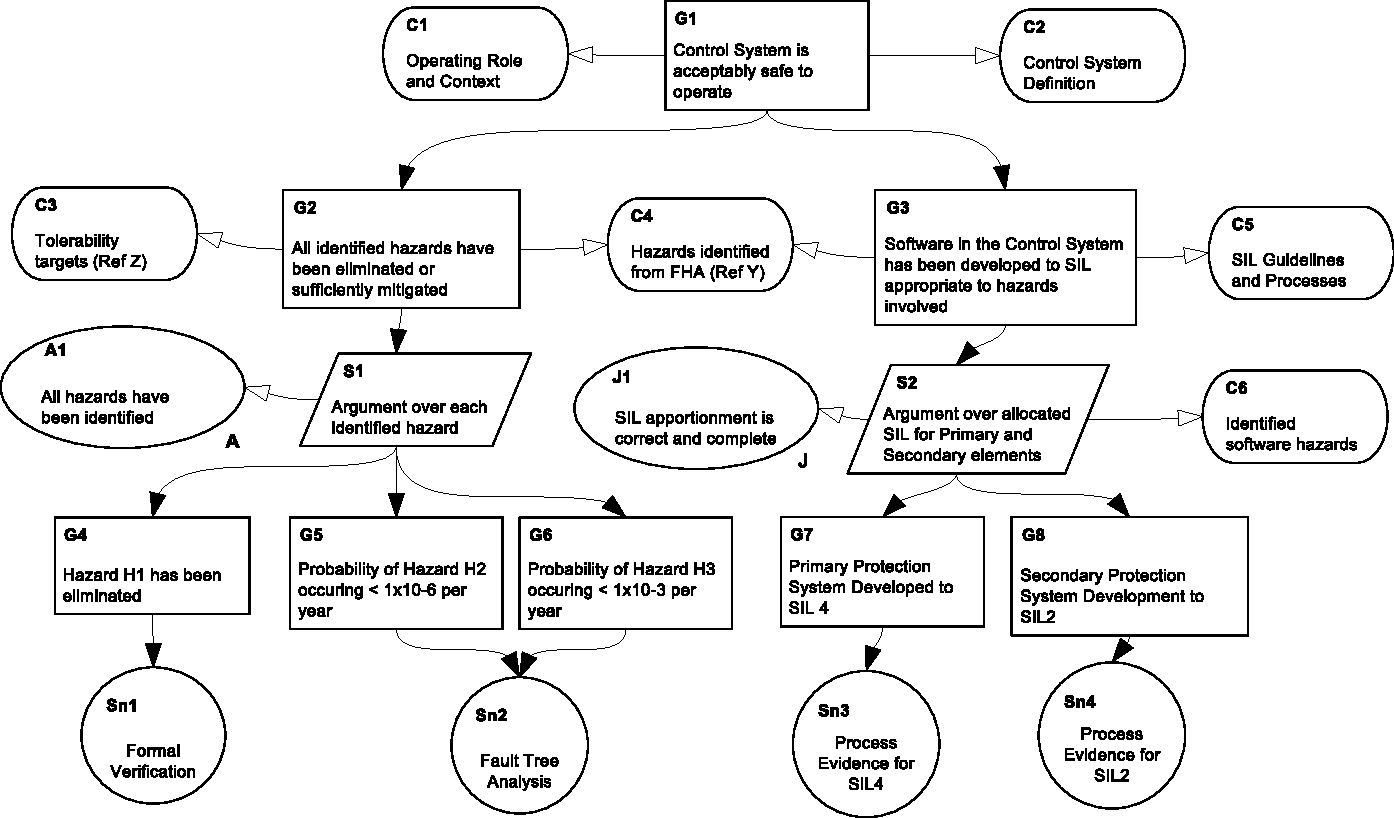
\includegraphics[width=\textwidth]{graphics/example_argument.pdf}
  \caption{An example GSN argument, about a safety case,
    from the GSN specification \cite{gsnstandard}}
  \label{fig:crampedex1}
\end{figure}




\section{Artoo}

\begin{figure}
  \centering
  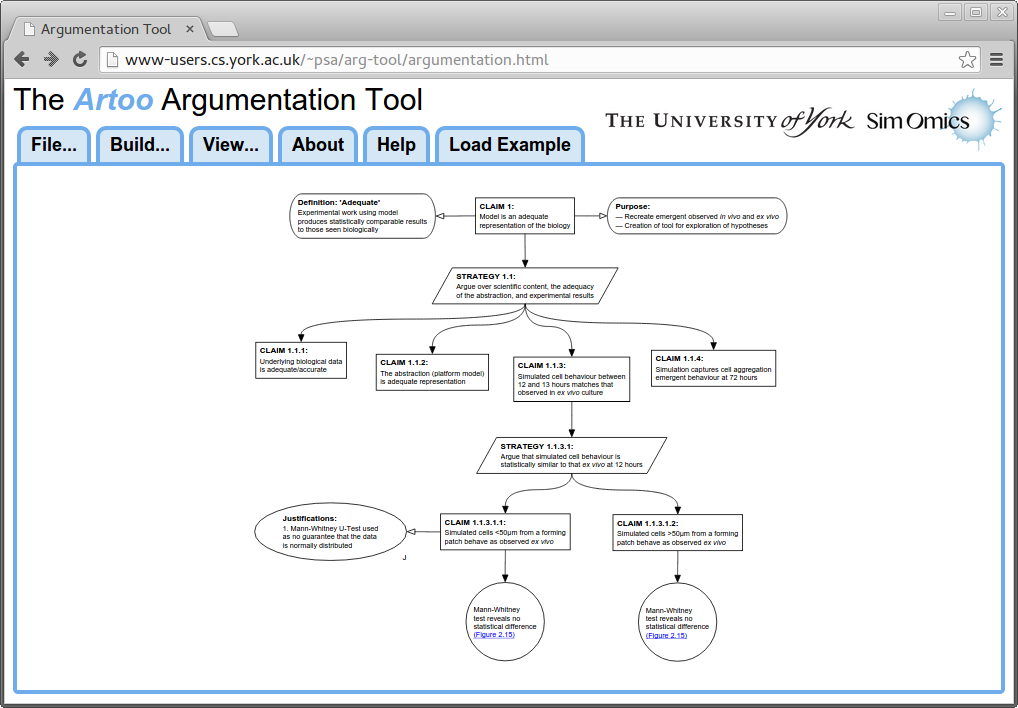
\includegraphics[width=\textwidth]{graphics/artoo_screenshot.png}
  \caption{The Artoo tool, displaying an argument}
  \label{fig:artoo}
\end{figure}

Artoo (Argumentation Tool) is a tool for drawing graphical structures, specifically using the GSN syntax.
It was developed by Paul Andrews at the York Computational Immunology Lab, and \citet{royal} introduce it with specific reference to using the GSN for arguing about biological simulations (which they demonstrate).

Artoo is a single-page, client-side web application, written in JavaScript, and runs in recent versions of most popular web browsers.
Arguments are displayed as Scalable Vector Graphics (SVG) documents embedded in the web page, can be downloaded as XML documents (containing all information about arguments' structure, semantics, content, and layout) which can be re-opened later, and can be exported as bitmap images.
Figure~\ref{fig:artoo} shows the tool displaying a GSN argument.\ldots

Artoo is available for free under a GNU GPLv3 licence.
This means that anyone can use it, view the source code, and modify it, within the terms of the license.
Other tools also exist for drawing GSN arguments, but they are typically commercial and closed-source, \todo{and so\ldots ?} and specifically emphasise the use of argumentation for presenting safety arguments.
Examples include Dependable Computing's
Argument Editor\footnote{\url{http://www.dependablecomputing.com/tools/index.html} \label{fn:depcomp}}
, and Adelard's
ASCE \footnote{\url{http://www.adelard.com/asce/choosing-asce/index.html}}.


\section{Motivation}

Currently, users of Artoo have full control over the layout of arguments they draw, and have to position each node on the infinite canvas using a pointing device.
(Edges are drawn automatically, based on connections defined by the user.)
Clearly, this becomes time-consuming and difficult to manage for larger arguments, and is made harder by the absence of features such as ``snap to grid'' [\ldots].
Furthermore, users may sometimes perform manual layout badly, an idea explored in section~\ref{sec:humangold}.

For these reasons, graph drawing tools often include automatic layout features.
In the area of argumentation, Dependable Computing's Argument Editor\footref{fn:depcomp} is one such tool. 
Other more general tools with automatic graph layout capabilities include [yWorks\ldots]


\section{Objectives and problem definition}

This project aims to add an automatic layout feature to Artoo.
Determining how this feature should work -- both at a high and low level -- will be important.

The process will involve researching and implementing various graph layout algorithms,
and testing them in a structured, repeatable way in order to compare them. 

Typically, a graph layout algorithm takes as its inputs a set of nodes and a set of edges, and outputs the positions 
In the case of a GSN argument, there is  information associated with the input graph:

\begin{itemize}
  \item
    Each node has a width and a height, whereas in the simplest model of a graph nodes are single points. \todo{,?}
  \item
    There are various types of node and edge, and the type of a node should influence where it is placed. Specifically: goals, strategies and solutions should be treated differently to context, assumption and justification elements.
    \begin{itemize}
    \item The GSN specification's layout guidance \citep[section~2.2, pp.~26--27]{gsnstandard} recommends that parent and child goals, strategies and solutions are placed above and below each other; context, assumption and justification elements should be placed to the left and right of their parents (helping to alleviate the problem of cross-references disrupting the flow of arguments).
    \end{itemize}
\end{itemize}

The paths of edges may also be outputted by non--straight line drawing algorithms. As Artoo already automatically draws edges depending on the positions of nodes, only the nodes' positions will be considered in this project.


\section{Structure}

\begin{itemize}
\item The \textbf{introduction} introduces the problem, the report and its structure.
\item \textbf{Research} discusses approaches to the layout of graphs, and approaches to evaluating their layout.
\item Decide on
\item
\item
\end{itemize}


\section{Statement of ethics}

There are few ethical considerations in this project.

Where third party open source software has been used, this has been made clear, and the license has been followed, with the relevant copyright and permission notices left intact in comments in the source code.

\begin{itemize}
\item Artoo: copyright \copy 2013 University of York, distributed under the terms of the GNU General Public License\footnote{\url{http://www.gnu.org/licenses/}} version 3
\item Springy: MIT License\footnote{\url{http://opensource.org/licenses/MIT}}
\item Arbor: MIT License
\item Dagre: MIT License
\end{itemize}

Although it is possible that argumentation and Artoo could be used to support unethical activities, this is beyond the scope of this project.
